% Completa los datos convenientemente en las zonas marcadas con TODO

\documentclass{beamer}
%PARA VISUALIZAR PRESENTACIONN CON NOTAS USAR VISUALIZADOR "pdfpc":
%Para ver las notas, el cronometro y siguente diapo:
% pdfpc --notes=right slides.pdf
% "tecla p": para pausar el cronometro
\mode<presentation> {
  \usetheme{Boadilla}
  \usecolortheme{rose}
}

\setbeamertemplate{navigation symbols}{} % ocultar iconos de navegación
\setbeamerfont{subsection in toc}{size=\small} % reducir tamaño en TOC
\setbeamerfont{date}{size=\tiny}
\usepackage[spanish]{babel}
\usepackage[utf8]{inputenc}
\usepackage{graphicx}
\usepackage{caption}
\usepackage{subcaption}
\graphicspath{ {figs/} }
\usepackage{booktabs}

\usepackage{hyperref}
\usepackage{multicol}
\usepackage{media9}
\usepackage{pgfpages}
\usepackage{listings}
\usepackage{multimedia}
\usepackage[export]{adjustbox}
\usepackage{outlines} % Para poner bullets tabulados (\1 \2 \3 ...) y no items

\usepackage{array,tabularx} % para tabular leyenda de ecuaciones
\newenvironment{conditions*} % entorno de "leyenda de ecuación"
  {\par\vspace{\abovedisplayskip}\noindent
   \tabularx{\columnwidth}{>{$}l<{$} @{\ : } >{\raggedright\arraybackslash}X}}
  {\endtabularx\par\vspace{\belowdisplayskip}}
  
% USO DE NOTAS
\setbeameroption{hide notes} % Para mostrar u ocultar (hide/show)
%\setbeameroption{show only notes} % Mostrar solo las notas
%\setbeameroption{show notes on second screen=right} % Mostrar notas en otra pantalla
\setbeamertemplate{note page}{ % asi solo muestro el texto de las notas
  \insertnote%
}

%========= TODO: datos internos del documento
\hypersetup{
	pdftitle={Defensa de Trabajo de Fin de Grado de Eva García Domingo},
	pdfauthor={Eva García Domingo},
	pdfsubject={Pon aquí el título completo del trabajo},
	pdfkeywords={teaching, robotics, sensors, actuators, python, scratch},
	pdfproducer={TeXStudio},
  colorlinks=true,
  linkcolor=blue
}
%=========

%========= TODO: diapositiva de portada
\title[Robótica Educativa]{Robótica Educativa con Python y mBot} % El título reducido aparece en la parte inferior de todas las diapositivas
                                         % El título completo aparece solo en la diapositiva de portada
\author[Eva García Domingo]{Eva García Domingo}
\institute[URJC]
{
\textit{\href{mailto:eva.garcia.domingo@gmail.com}{\color{blue}{\underline{eva.garcia.domingo@gmail.com}}}}\\
\vspace{0.5cm}

\includegraphics[width=3cm]{logo-urjc}\\
\vspace{1cm}
Trabajo Fin de Grado
}
\date{15 de Julio de 2022}
%=========

%========= COMIENZO DEL DOCUMENTO
\begin{document}

%========= Portada inicial con notas
\begin{frame}[plain] % plain: quita header y footer
\large{\titlepage}
\note[item]{En esta presentación vamos a hablar sobre robótica educativa con el robot mBot}
\note[item]{}
\end{frame}

%========= Licencia
\begin{frame}
% Este diseño se corresponde con la licencia CC-BY-NC-SA.
% Por supuesto, puedes poner la licencia que mejor se adapte al propósito de tu trabajo.
% Recuerda que, si no se especifica ninguna licencia, esta -como cualquier creación artística- pasaría a estar licenciada con todos los derechos reservados (copyright).

\vspace{5cm}

\begin{flushright}

\begin{figure}

\includegraphics[width=0.10\textwidth,right]{figs/by-nc-sa.png}
\end{figure}

\vspace{0.2cm}

{\tiny 
(CC) \textbf{Eva García Domingo}\\ % TODO: pon aquí tu nombre cuando hagas el documento
\vspace{0.5cm}
\emph{
Este trabajo se entrega bajo licencia \href{https://creativecommons.org/licenses/by-nc-sa/3.0/es/}{CC BY-NC-SA}. \\
Usted es libre de \textit{(a) compartir}: copiar y redistribuir el material en \\
cualquier medio o formato; y \textit{(b) adaptar}: remezclar, transformar \\
y crear a partir del material. El licenciador no puede revocar estas \\
libertades mientras cumpla con los términos de la licencia. \\}
}

\end{flushright}


\end{frame}

%========= Índice o tabla de contenidos (TOC)
\begin{frame}
\frametitle{Contenidos}
%\begin{multicols}{2} % si tengo muchas secciones, lo parte en dos columnas
  \tableofcontents[hideallsubsections] % no muestra subsecciones
%\end{multicols}
\note[]{}
\note[]{}
\end{frame}

%========= Diapositiva "vacía" de comienzo de sección:
\section{Introducción}

\subsection{Contexto general}
%========= Diapositiva con imágenes:
\begin{frame}
\frametitle{Introducción}
\framesubtitle{Situación de la Robótica}

	\begin{itemize}	
		\item Disciplina alejada del público
		\item Los últimos años ha empezado a cambiar: ``robots'' en la vida diaria (Bots, Internet Of Things, Inteligencia Artificial, Domótica, Ocio)
	\end{itemize}
\begin{columns}
	
	\begin{column}{0.5\textwidth}
		\centering
		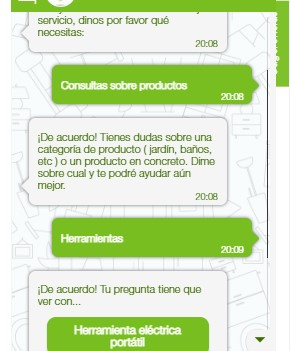
\includegraphics[height=3cm]{chatbot.jpg}
		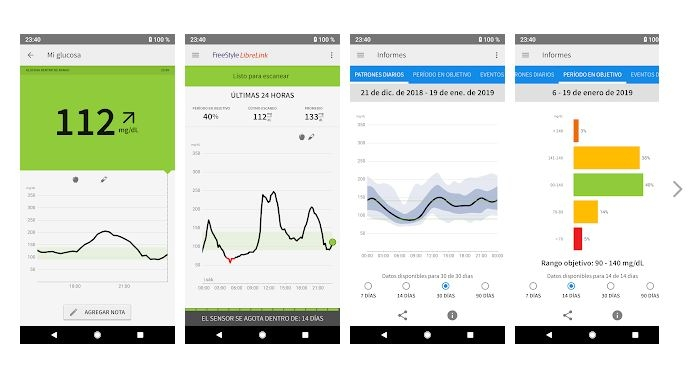
\includegraphics[height=3cm]{IOT3.jpeg}
	\end{column}
	\begin{column}{0.5\textwidth}
		\centering
		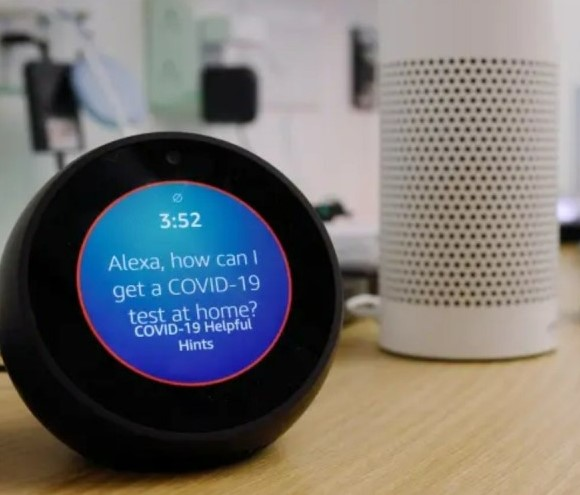
\includegraphics[height=3cm]{alexa.jpg}
		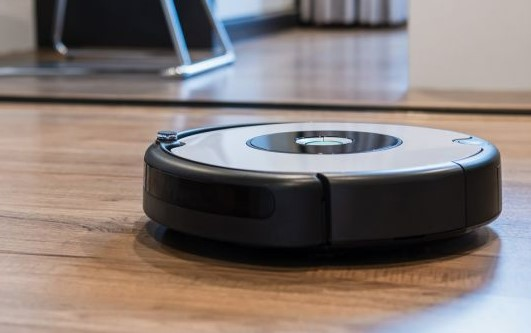
\includegraphics[height=3cm]{domotica1.jpg}
	\end{column}

	
\end{columns}
	\note[item] {Es vista como una asignatura muy compleja, sólo accesible a grandes corporaciones, tanto por poder adquisitivo como por recursos académicos. Además, muy asociada a la ciencia ficción, la idea de robot está muy alejada de la realidad}
	\note[item]{La ingeniería, y el mundo comercial, han cambiado poco a poco el concepto de la sociedad tiene de la robótica, como disciplina, y de los robot. }
	\note[item]{Las diferentes facetas de la robótica tienen cada vez más ejemplos en nuestra vida diaria, lo que ha contribuido a que las personas dejen de considerarlo ajeno o de ciencia ficción. Desmitificar una disciplina significa despertar el interés del publico en general en ella a la que dedicarse, tanto educativa como profesionalmente.}
\end{frame}

\begin{frame}
\frametitle{Introducción}
\framesubtitle{Situación de la Robótica}
\begin{itemize}
		\item  Cuanta más gente pueda acceder a los recursos necesarios, mejor

	\begin{figure}
		\centering
		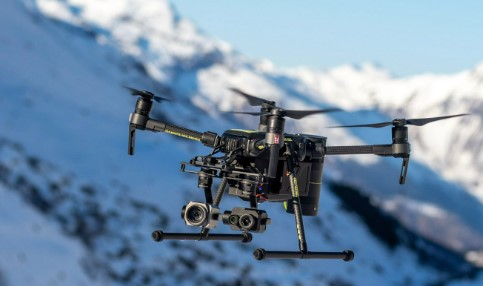
\includegraphics[width=0.33\textwidth]{droneski.jpg}
		\hspace{1cm}
		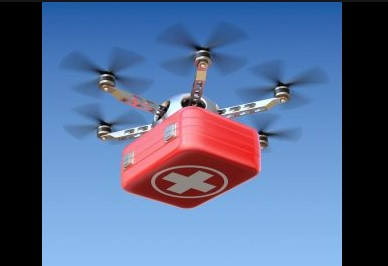
\includegraphics[width=0.33\textwidth]{dronerescate.jpg}
	\end{figure}

\item La forma de conseguir expandir la robótica es empezar desde jóvenes
\item La programación y el pensamiento computacional es algo muy complejo si se empieza en etapas educativas avanzadas
\end{itemize}
	\note[item]{ Ha sido muy importante que el acceso a recursos y componentes se haya extendido. Cuánta más gente pueda dedicarse a ello, más posibilidades se abrirán y más aplicaciones prácticas en todos los ábmbitos. Al no ser una disciplina extendida, quizá nadie había reparado en una aplicación concreta.}
	\note[item]{Por ejemplo, con un drone, podemos pasar de tener un elemento de ocio con el que grabar un espectáculo deportivo, a mandar ayuda humanitaria a sitios a los que de otra forma no podríamos llegar - o no llegaríamos a tiempo.}
\end{frame}

\subsection{Contexto específico}

\begin{frame}
	\frametitle{Introducción}
\framesubtitle{Antecedentes}
\begin{block}{Robótica Educativa}
	\begin{itemize}
		\item Open Roberta
		\item Lego Boost
		\item Kibotics
		\item mBlock
	\end{itemize}
\end{block}

\begin{block}{Antecedentes en la URJC}
	Organización JdeRobot y PyBoKids
\end{block}
\begin{block}{Experiencia práctica}
	Curso escolar de clases extracurriculares
\end{block}
\end{frame}

\section{Objetivos}
\begin{frame}
\frametitle{Objetivos}
\begin{block}{Infraestructura para la programación en Python}
	\begin{itemize}
	\item Programación en Python
	\item Funcionalidad oculta al estudiante
	\item API de fácil accesibilidad
	\item Biblioteca en Arduino a bordo del mBot
	\end{itemize}
\end{block}

\begin{block}{Propuesta educativa basada en Scratch y Python}
	\begin{itemize}
		\item Robot educativo mBot
		\item Plataformas del fabricante y la nuestra en Python
		\item Ejercicios escalonados en dificultad y con objetivos docentes a corto, medio y largo plazo
	\end{itemize}
\end{block}
\end{frame}

\section{Herramientas usadas}
\begin{frame}
\frametitle{Herramientas usadas}


\begin{columns}
	\begin{column}{0.5\textwidth}
		\begin{figure}
		\centering
		
\includegraphics[height=2cm]{Windows.jpg}
		\end{figure}
		\begin{figure}
			\centering
			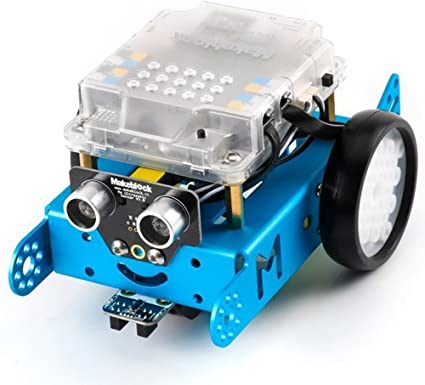
\includegraphics[height=2cm]{mbot.jpg}
		\end{figure}
		\begin{figure}
			\centering
			
\includegraphics[height=2cm]{scratch-logo.png}
		\end{figure}
	\end{column}
	\begin{column}{0.5\textwidth}
		\centering
		\begin{figure}
		\centering
		
\includegraphics[height=3cm]{arduino-logo.png}
		\end{figure}
		\begin{figure}
			\centering
		
\includegraphics[height=3cm]{python-logo.png}
		\end{figure}
	\end{column}
\end{columns}

\note[item]{El objetivo de todas las elecciones de infraestructura ha sido la accesibilidad de ellas}
\note[item]{el sistema operativo windows es el más extendido y conocido, siendo Linux más visto como académico y complicado. Si queremos interesar a los jóvenes, y facilitar su acceso a los recursos, utilizar los recursos que ya conocen es una ventaja}
\note[item]{Las placas Arduino son las más extendidas, por estar diseñadas particularmente para la enseñanza y su bajo coste. El proyecto es open source, por lo que hay mucho contenido para ellas.  El robot contiene una gran cantidad de sensores y actuadores muy útiles para la robótica educativa: comentar los sensores y actuadores}
\note[item]{Scratch es un lenguaje de programación en bloques, muy visual y perfecto como primera aproximación a la programación. Podemos enseñar conceptos de programación como funciones o variables, pensamiento computacional o Algoritmia sin tener que recurrir a un lenguaje textual de programación clásica, mucho más complejo por sus normas (sintaxis, compilación, ejecución, etc) }


\end{frame}
\section{PyBoKids 2.0}
\subsection{Diseño}
\begin{frame}
	\frametitle{Diseño}
	\framesubtitle{Diseño general del modelo PC - Residente}
	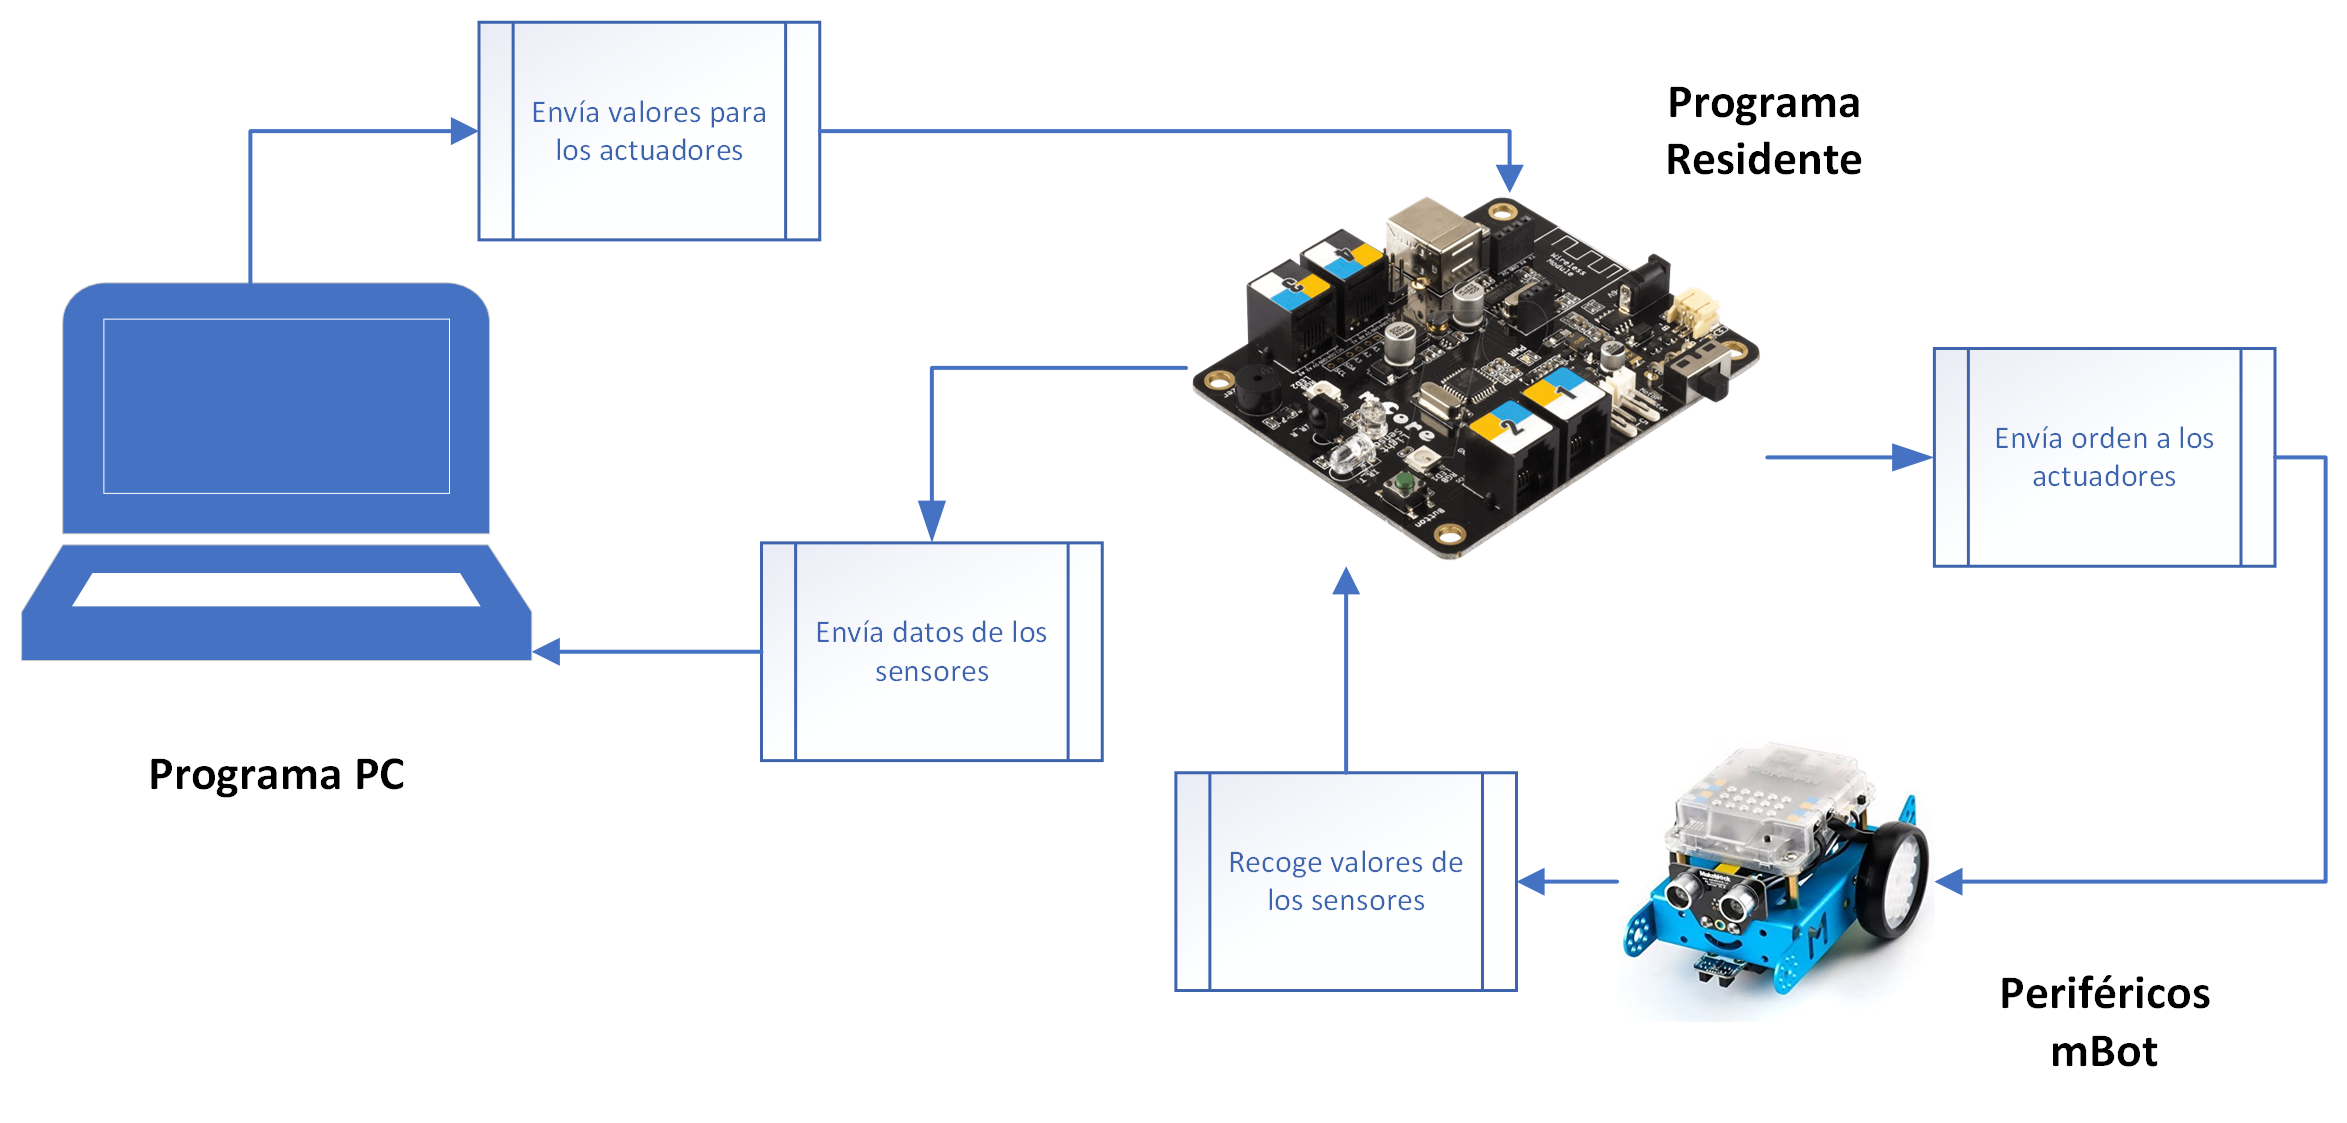
\includegraphics[width=\textwidth]{flujo1-1.png}
	
	
	\note[item]{era necesaria una forma para que, ya que la placa base funciona en Arduino, la comunicación Serial1 funcionara entre los dos lenguajes.
	El diseño realizado consta de tres partes: el robot mBot, el PC y las comunicaciones en vivo entre ambos. El software desarrollado ofrece en el PC una biblioteca para que la aplicación
	principal, que se ejecuta en el ordenador, acceda en vivo a los sensores y actuadores del robot,
	a través de la aplicación que se ejecuta en su placa base}
	\note[item]{El programa residente recoge los valores de los sensores, conectados a su puerto correspondiente, y los envía por el canal}
	\note[item]{El programa PC recoge los valores del sensor que le interese (si así lo programamos)}
	\note[item]{El programa PC envía por el canal unos valores concretos para un actuador concreto (con respecto a lo leído de los sensores o no)}
	\note[item]{El programa residente lee del canal si tiene mensajes para un actuador y, en caso afirmativo,	recoge los valores y los envía al actuador correcto}
\end{frame}

\begin{frame}
	\frametitle{Diseño}
	\framesubtitle{Comunicación por mensajes}
	\large{La información debe ser \textcolor{blue}{inequívoca}}
	\includegraphics[width=\textwidth]{mensajesensor.png}
	\includegraphics[width=\textwidth]{mensajeactuador.png}
	
	
	
	
	\note[item]{Para que la comunicación entre el programa PC y Residente sea posible es necesario un
		protocolo de mensajes; es necesario asegurarse que ambas partes recojan la información correcta y sepan qué deben hacer con ella.}
	\note[item] {Esta lógica de comunicaciones será invisible para el estudiante, ''escondida'' en la API.}
	\note[item]{El programa residente debe estar preparado para \textcolor{blue}{entender} los datos que recibe para los actuadores}
	\note[item]{El programa PC debe enviar esa información de forma \textcolor{blue}{inequívoca}}
	\note[item]{Igualmente para los sensores: el programa residente debe enviar los datos de forma que el PC sepa sin lugar a dudas \textcolor{blue}{a qué sensor} le corresponde ese dato}
	\note[item]{Esto lo conseguimos asignando identificadores numéricos a cada sensor/actuador}
\end{frame}



%========= Diapositiva con códigos:
\subsection{Desarrollo}
\begin{frame}
	\frametitle{PyBoKids 2.0}
	\framesubtitle{Programa Residente}
	Esta biblioteca está grabada en la placa base del robot y se ocupa de funcionar bajo todas las posibilidades
	\vspace{1cm}
	\begin{columns}
		\begin{column}{0.5\textwidth}
			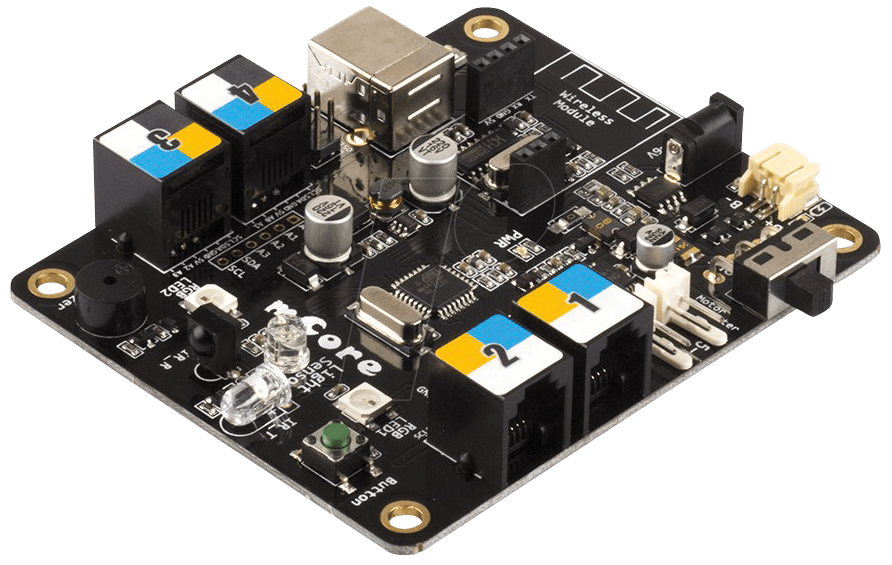
\includegraphics[width=0.7\columnwidth]{mcore.png}
		\end{column}
		\begin{column}{0.5\textwidth}
			\begin{enumerate}
				\item Manejo de sensores y actuadores
				\item Control de apagado
				\item Comunicaciones
			\end{enumerate}
		\end{column}		
	\end{columns}
\end{frame}


\begin{frame}
	\frametitle{PyBoKids 2.0}
	\framesubtitle{Programa PC}
	\begin{columns}
		\begin{column}{0.5\textwidth}
			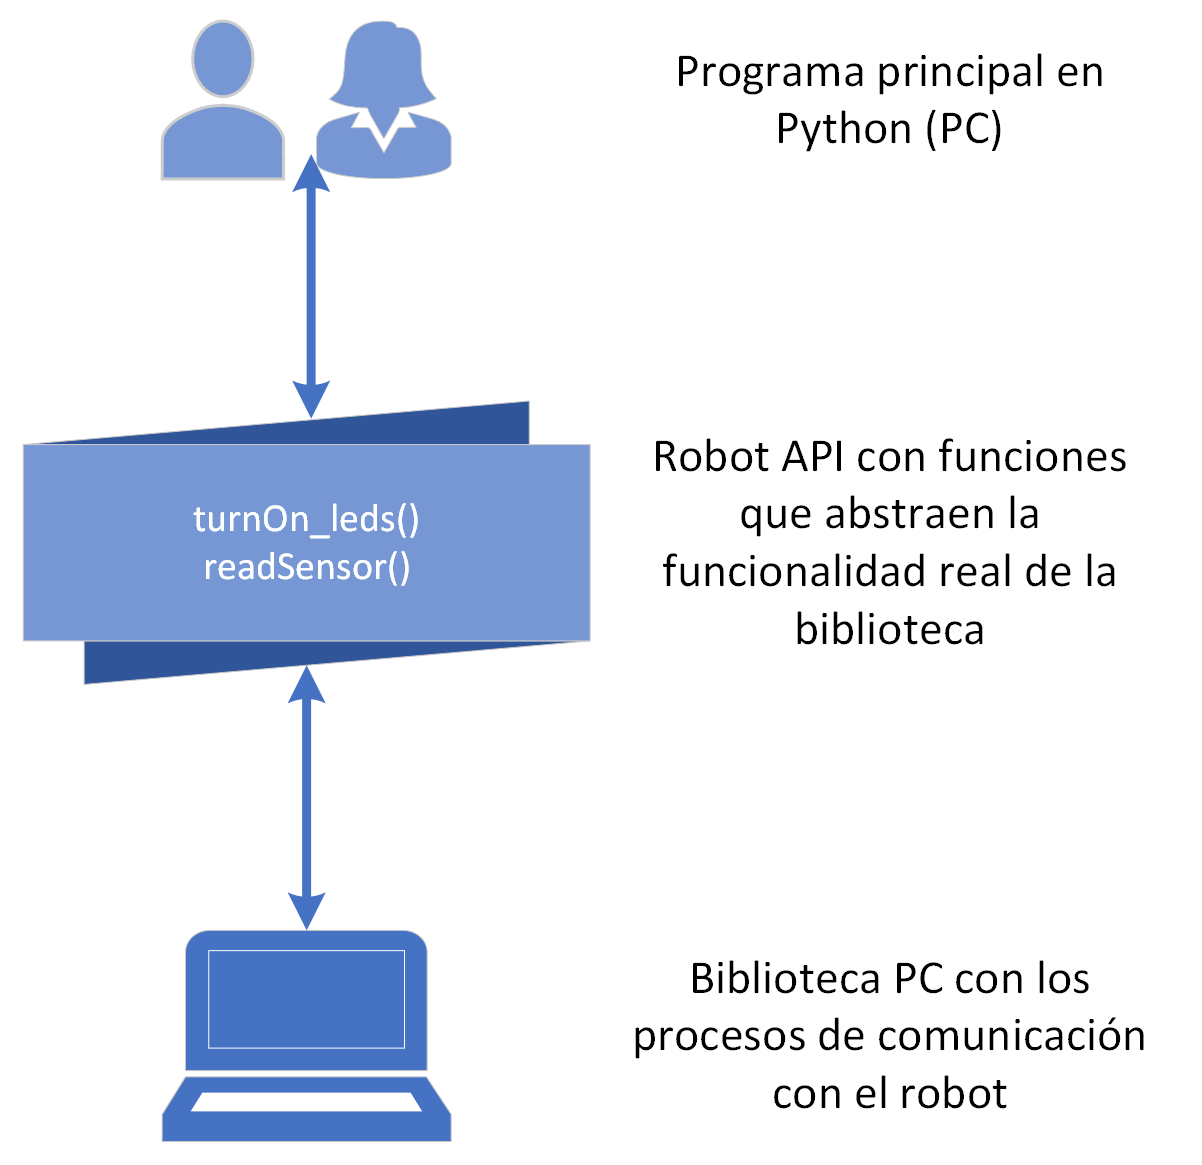
\includegraphics[width=1\columnwidth]{abstraccionPC.png}
		\end{column}
		\begin{column}{0.5\textwidth}
			\begin{enumerate}
				\item Manejo de sensores y actuadores
				\item Control de apagado
				\item Comunicaciones
			\end{enumerate}
		\end{column}		
	\end{columns}

\note[item]{Con esta biblioteca, abstraemos toda la lógica, tanto de comunicaciones con el mBot como las particularidades de la sintaxis más ''farragosa''. El objetivo es ofrecerle al estudiante funciones sencillas y autoexplicativas}
\end{frame}

\begin{frame}
	\frametitle{PyBoKids 2.0}
	\framesubtitle{Ejemplo de uso}
\begin{figure}
	\centering
	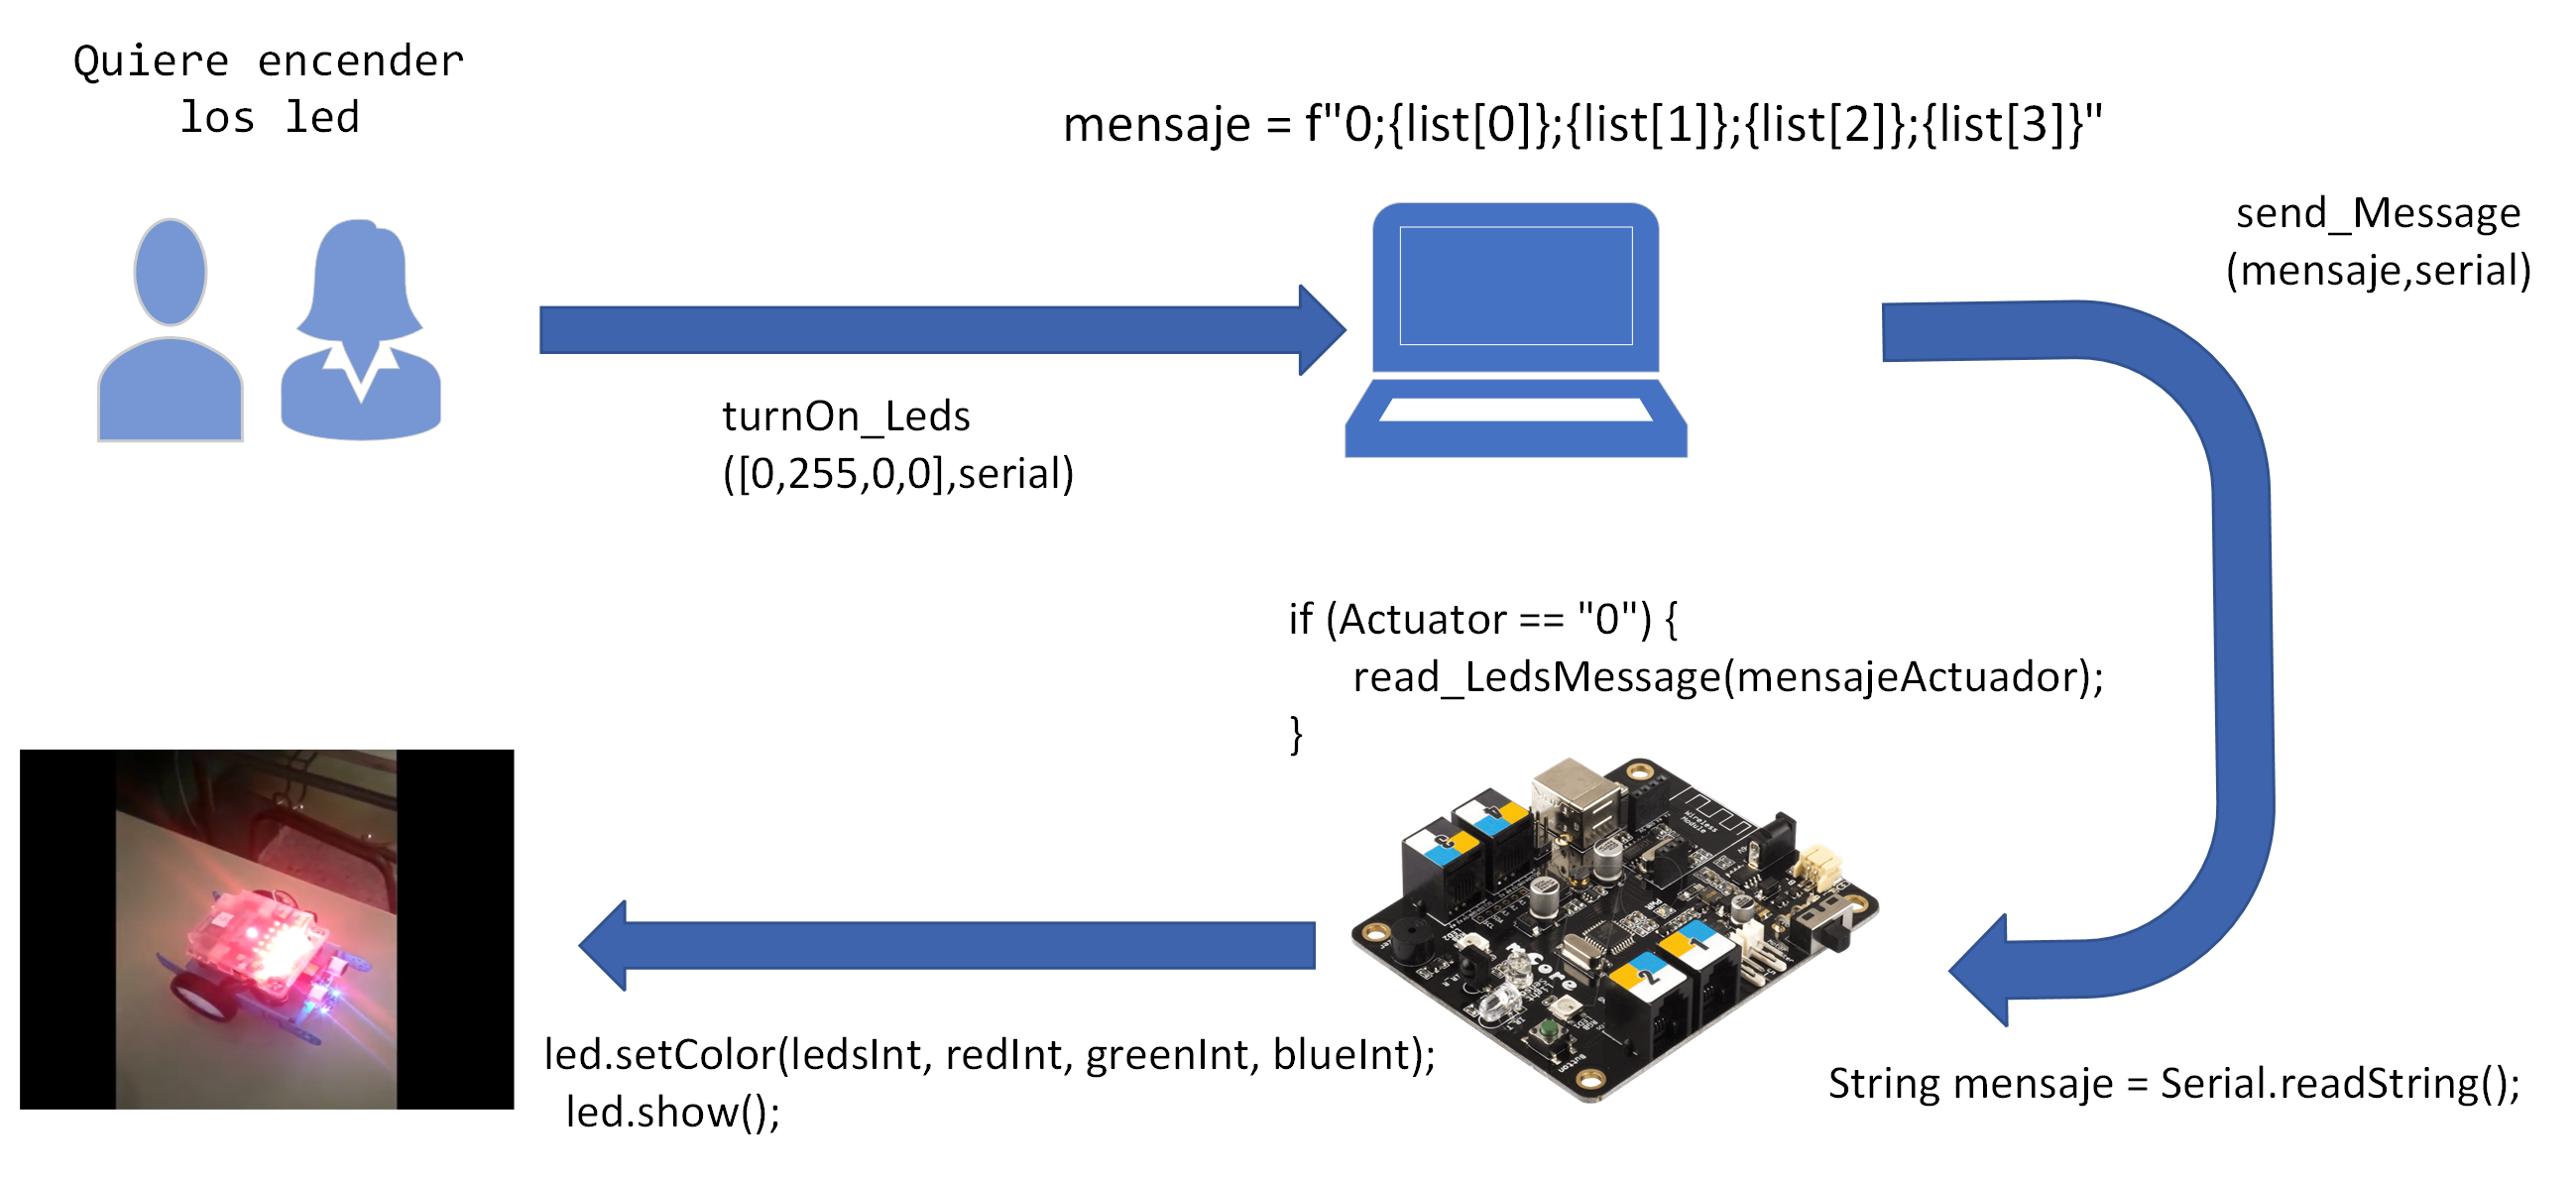
\includegraphics[width=\textwidth]{ejemplo.png}
\end{figure}
		
		\note [item]{Desde el programa principal, el alumno envía los datos necesarios para encender los motores. Para ello, recoge los datos de teclado, y utiliza la función ``visible'' de la API}
		
		\note [item]{La función \textit{turnOn\_Motors} de la biblioteca Python, contiene la lógica de codificación y envío a través del canal Serial}
		\note [item]{En el programa residente, se lee del canal que hay datos disponibles, y decodifica a qué actuador le corresponde el mensaje}
		\note [item]{A la función le llega solo los datos que necesita para el actuador, que decodifica y envía a los motores}

\end{frame}



\section{Contenidos educativos}

\begin{frame}
\frametitle{Contenidos Educativos}
\framesubtitle{Scratch y mBlock}

	\begin{block}{}
		\begin{itemize}
			\item Scratch: lenguaje de bloques
			\item Objetivos: conceptos y metodologías de forma gradual
			\item Prácticas: aplicaciones ``reales'' con objetivos docentes especificados
		\end{itemize}
	\end{block}	
\end{frame}

\begin{frame}
	\frametitle{Contenidos Educativos}
	\framesubtitle{Scratch y mBlock}
	Programar un sistema de luces automáticas de un coche; \textcolor{blue}{variables}, \textcolor{blue}{condiciones de entorno}, \textcolor{blue}{bucles} y \textcolor{blue}{condicionales}.
	\newline
	\begin{columns}
		\begin{column}{0.7\textwidth}
			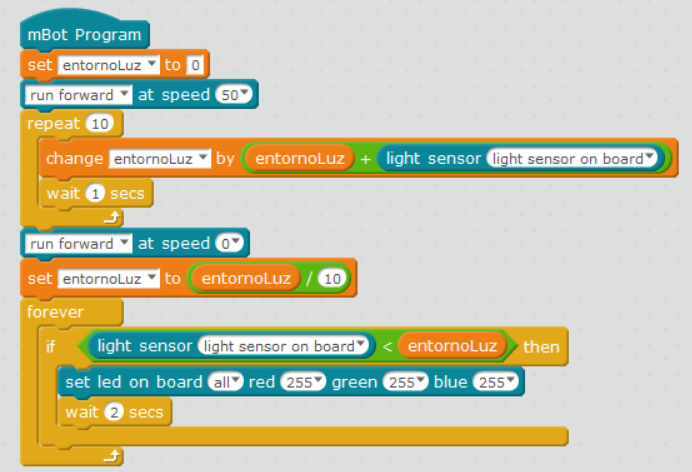
\includegraphics[width=\columnwidth]{lucesautomaticas.png}
		\end{column}
		\begin{column}{0.30\textwidth}
			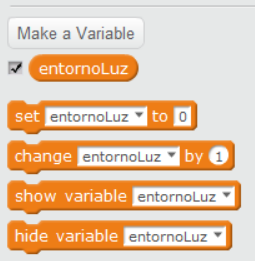
\includegraphics[width=\columnwidth]{variableLuz.png}
		\end{column}
	\end{columns}
\end{frame}

\begin{frame}
\frametitle{Contenidos Educativos}
\framesubtitle{Python}
	\begin{block}{Objetivos}
		\begin{itemize}
			\item Lenguaje textual más cercado a la programación real
			\item API de PyBoKids-2.0
			\item Añadir un grado de complejidad de forma natural
		\end{itemize}
	\end{block}
\begin{block}{Prácticas}
	\begin{itemize}
		\item Pequeño curso introductorio al lenguaje 
		\item Ejercicio \emph{esqueleto.py} para ayudar en la transición 
		\item Soluciones de referencia a los principales ejercicios
		\item Añade la posibilidad de interactuar en tiempo real con el robot
		\item Limitadas a tener conectado el robot por USB al PC
	\end{itemize}
\end{block}
\end{frame}
\begin{frame}
\frametitle{Contenidos Educativos}
\framesubtitle{Python}
	Ejercicio introductorio para el sensor de ultrasonidos, en el que el robot estará ``en verde'' si no tiene un obstáculo delante, y ``rojo'' en caso contrario.
	\begin{figure}
		\centering
		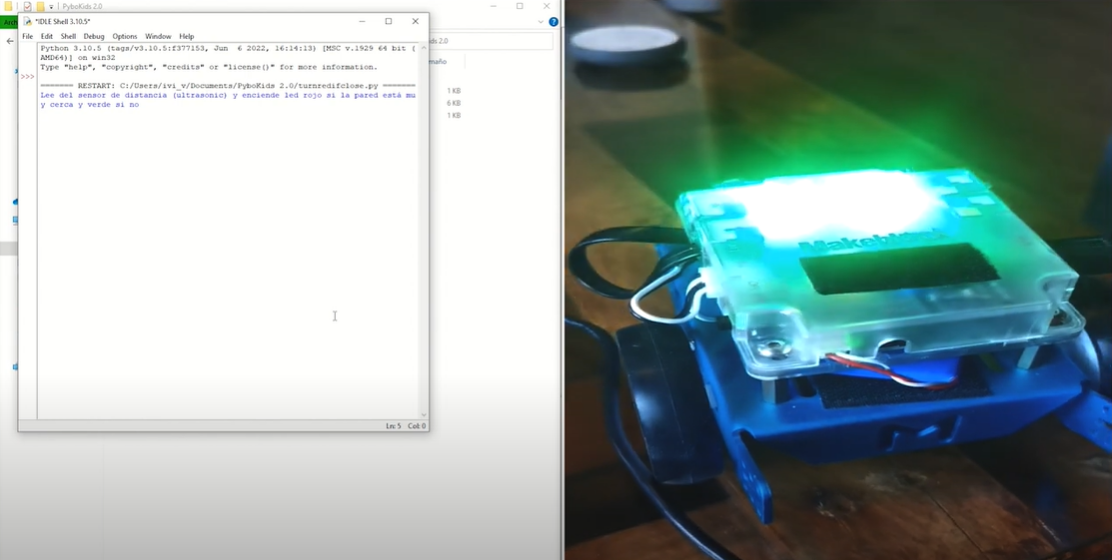
\includegraphics[width=\textwidth]{ejemplopython.png}
	\end{figure}
\end{frame}

\section{Conclusiones}


\begin{frame}
	\frametitle{Conclusiones}
	\begin{block}{Objetivos cumplidos}
		\begin{itemize}
		\item \textit{Middleware} para programar el mBot en Python que abstrae la dificultad del lenguaje y del Arduino nativo del robot
		\item No requiere de programación en Arduino, ni de la instalación de nada excepto Python para el uso de la biblioteca
		\item Esto hace que sea posible utilizarla fácilmente en clases de robótica educativa, teniendo en cuenta los recursos limitados de los centros educativos
		\item Propuesta educativa completa con objetivos individuales y colectivos, orientado principalmente a Educación Primaria y Secundaria, que responden a una experiencia práctica
		\end{itemize}
	\end{block}

	
\end{frame}

\begin{frame}
	\frametitle{Conclusiones}
	\begin{block}{Líneas futuras}
		\begin{itemize}
			\item Ampliar los sensores y actuadores en las bibliotecas
			\item Añadir funcionalidad Bluethooth a la solución
			\item Adaptar la infraestructura para hacer posible la elección de periféricos desde el programa principal
		\end{itemize}
	\end{block}
\end{frame}

\begin{frame}[plain]
\large{\titlepage}
\note[item]{Y hasta aquí mi exposición.}
\note[item]{Quedo a disposición del tribunal...}
\end{frame}

\end{document}
